\documentclass{article}

% Language setting
% Replace `english' with e.g. `spanish' to change the document language
\usepackage[UTF8]{ctex}

% Set page size and margins
% Replace `letterpaper' with `a4paper' for UK/EU standard size
\usepackage[letterpaper,top=2cm,bottom=2cm,left=3cm,right=3cm,marginparwidth=1.75cm]{geometry}

% Useful packages
\usepackage{amsmath}
\usepackage{graphicx}
\usepackage[colorlinks=true, allcolors=blue]{hyperref}

\title{Calculation Geophysical Dynamic Fluid}
\author{Wang ZY} % Your name

\begin{document}
\maketitle
\tableofcontents
\newpage

\section{基础知识}
\subsection{计算流体力学的基本定义}
地球流体力学方程:地球流体运动一般可用一组偏微分方程来描述,包括作为因变量的流场变量和作为自变量的时空坐标;

地球流体力学方程的特征:往往是非常复杂的和非线性的,根本不知道是否有通解存在。为了获得对地球流体运动物理特性的了解,非常必要去发展数值方法以求得近似解。

计算地球流体力学:专门研究求解地球流体力学方程的数值方法及其相关理论(季仲贞等1999;2000),是近四十年里发展起来的地球流体力学的一个分支学科。计算地球流体力学为大气模式和海洋模式动力框架的建立提供数值算法;动力框架在大气模式和海洋模式中扮演着发动机的角色;大气模式和海洋模式是气候系统模式最主要的分量模式,是气候数值模拟的重要工具。

\subsection{线性赋范空间}
\subsubsection{集合}
把若干确定的有区别的(不论是具体的或抽象的)事物合并起来,看作一个整体,就称为一个集合,其中各事物称为该集合的元素(Cantor, 1873年12月7日);

\subsubsection{线性空间}
对于一个给定的集合A,$\forall a,b\in A, \beta\in R$, 如果$a\oplus b\in A, a\otimes\in A$,则集合A就被称之为一个线性空间;

线性空间不同于集合的地方是它涉及到了两个运算,即加法和数乘运算;这两个运算可以是通常意义下的加法和数乘,也可以是自己定义的加法和数乘。

加法运算需要满足:加法交换率:$a\oplus b = b \oplus a$;

加法结合率: $a \oplus (b \oplus c) = (a \oplus b) \oplus c $;

零元素:集合中存在“零元素”o,使得$a \oplus o = a $;

逆元素:集合中任意一个元素a存在“逆元素”$\chi$,使得 $a\oplus \chi = o$ ;

数乘运算需要满足:

数乘结合律:$(a \otimes \beta ) \otimes \gamma= a \otimes (\beta \times \gamma)$;

与实数1的数乘:$a \otimes 1= a$ ;

第一分配律: $a \otimes (\beta + \gamma) = (a \otimes \beta) \oplus (a \otimes \gamma ) $;

第二分配律: $(a \oplus b) \otimes \beta = (a \otimes \beta) \oplus (b \otimes \beta )$

\subsubsection{线性子空间}
设V是一个线性空间,W是V的一个非空子集,对于V的加法和数乘运算,W也构成一个线性空间,则W为V的一个线性子空间,记为$W\subseteq V$;

设W是V的线性子空间,且W为 V的真子集,则W为V的真子空间,记为$W\subset V$。

\subsubsection{范数}
设X为一个线性空间。$\forall x \in X$,都有一个被记作‖x‖的实数与它对应,且满足:

$‖x‖\ge 0, ‖x‖=0 \leftrightarrow x=0 $(零元素);

$\forall x\in X, \alpha\in R,  ‖\alpha x‖=|\alpha|‖x‖$;

$\forall x,y\in X, ‖x+y‖\le‖x‖+‖y‖$ (三角不等式);

\subsubsection{线性赋范空间}
定义了范数的线性空间称为线性赋范空间或简称赋范空间。

\subsubsection{Banach空间}
若X中的任何收敛序列${x_n}$的极限仍然在X中,即存在$x_0\longrightarrow X$,使得$d(x_n,x_0)\longrightarrow 0$,则称X是完备的线性赋范空间,又称为Banach空间。

\subsection{Hilbert空间}

\subsubsection{内积}
设X是一个线性空间,若$\forall x,y\in X, \alpha\in R$,总有按某种法则对应的一个实数(x,y),满足三个条件:

1. 齐次性:$(\alpha x,y)=\alpha(x,y)$;

2. 对称性:$(y,x)=(x,y)$;

3. 非负性:$(x,x)\ge0$,且(x,x)=0等价于x=0;

\subsubsection{Hilbert空间}
设X是一个内积空间,若由它的内积派生的范数下,X是个完备的线性赋范空间,即Banach空间,则称X是完备的内积空间,或称为Hilbert空间。

\subsection{线性算子与线性泛函}
设X和Y是函数空间, $D_T$和$S_T$分别是X和Y的子集,$\forall x(t)\in D_T$,都按照某一规则有确定的$S_T$中的一函数y(t)与之对应,则称在$D_T$上定义了一个算子T,记作y=Tx。 $D_T$称为T的定义域, $S_T$称为T的值域。

\subsubsection{线性算子}
设T为定义在$D_T$上的算子, $\forall x,x_1,x_2\in D_T,\alpha\in R$,T满足:

1. $T(x+y)=Tx+Ty$

2. $T(\alpha x) = \alpha Tx$

则算子T为一线性算子。

\subsubsection{线性泛函}
线性泛函是一个特殊的线性算子。

若$\forall x\in D_f\subset X$(X为函数空间),都按照某一规则有确定的一实数$y\in R_f\subset R$( R为实数集)与之对应,则称在$D_f$上定义了一个泛函f ,它对$\forall x,y\in D_f,\alpha\in R$,满足

1. f(x+y)=f(x)+f(y)

2. $f(\alpha x)=\alpha f(x)$

\subsubsection{伴随算子}
设$M_1,M_2\subset X$, X为Hilbert空间, A为$M_1$到$M_2$的一个线性算子,若$\forall u \in M_1,v\in M_2$,存在$M_2$到$M_1$的线性算子$A^∗$,使得对配备在X上的内积$(\cdot,\cdot)$,满足:$(Au,v)=(u,A^∗v)$,则称$A^∗$是A的伴随(共轭)算子,当A为实数矩阵时,其伴随也记为$A^T$

\subsubsection{对称算子和反对称算子}
设$A^∗$是A的伴随(共轭)算子,若$A^∗=A$,则称A为对称算子,或自伴随(自共轭)算子;

若$A^∗=−A$,则称A为反对称算子;

若A为线性算子,则A为反对称算子的充分必要条件是:(Au,u)=0;

利用(Au,u)=0,可以定义非线性算子的反对称性。

\subsubsection{广义反对称算子}
若A为线性或非线性算子,若A满足(Au,u)=0;则A为广义反对称算子,简称反对称算子。广义反对称是反对称在非线性情形的推广。

\subsubsection{耗散算子和反耗散算子}
A是一个线性或非线性算子,如果A满足:(Au,u)<0,则称A为耗散算子;

如果A满足:(Au,u)>0,则称A为反耗散算子,也叫正定算子或正算子。

\subsection{发展方程}
齐次发展方程:
$$\frac{\partial F}{\partial t} + LF = 0$$

非齐次发展方程:
$$\frac{\partial F}{\partial t} + LF = G$$

\subsubsection{能量耗散、反耗散和能量平衡系统}
对于非齐次发展方程,若L为广义反对称算子:(LF,F) = 0,且有(G,F)<0,则称方程系统为一个能量耗散系统,即能量是衰减的。

对于非齐次发展方程,若L为广义反对称算子:(LF,F) = 0,且有(G,F)>0,则称方程系统为一个反能量耗散系统,即能量是增长的。

对于非齐次发展方程,若L为广义反对称算子:(LF,F) = 0,且有$\int_0^\infty(G,F)dt=0$,则称方程系统为一个能量平衡系统,即能量在长时间尺度上是平衡的。

实际的大气、海洋系统不是严格的能量守恒系统,因为有太阳的辐射强迫和地球自转的角动量输送;大气、海洋系统在演变过程中,存在局部的能量耗散(能量衰减),也存在局部的能量反耗散(能量增长),但整体来说,在长时间尺度上其能量收支是平衡的,即为能量平衡系统。

\subsubsection{发展方程的离散化}
考虑算子形式的齐次发展方程:
$$\frac{\partial F}{\partial t} + LF = 0$$

L为广义反对称算子,其离散化分二个步骤:

1)空间离散化,即构造与L相容的离散算子;(截断误差趋于0,见3.1.1)

2)时间离散化,即在空间离散化的基础上构造隐式、显式和半隐式全离散格式。

\subsubsection{半离散方程}
把发展方程中的空间微商算子L替换成与之相容的空间离散算子$\mathbf{L}$所得到的常微分方程,即为该发展方程的半离散方程:
$$\frac{d F}{d t} + \mathbf{L}F = 0$$


\subsubsection{反对称空间离散算子的构造}
1. Jacobian方法

Jacobian算子J[A,B],在水平方向上:
$$J[A,B] = \frac{\partial A}{\partial x}\frac{\partial B}{\partial y}-\frac{\partial A}{\partial y}\frac{\partial B}{\partial x}$$

正压涡度方程:
$$\frac{\partial \zeta}{\partial t}+J[\psi,\zeta]=0$$

Jacobian算子的双反对称性:

对于定义的内积:
$$(A,B) = \iint ABdxdy$$

不难验证,在周期或齐次边界条件下,无论对A还是B,Jacobian算子都是反对称的,即:
(J[A,B],A) = (J[A,B],B) = 0

事实上,由于Jacobian算子具有两种等价的通量散度形式,因此,在整个区域的积分为零(在周期或齐次边界条件下):
$$\iint J[A,B]dxdy = \iint \frac{\partial }{\partial x}(A\frac{\partial B}{\partial y})-\frac{\partial }{\partial y}(A\frac{\partial B}{\partial x})dxdy=0$$

而有$AJ[A,B] = \frac{1}{2}J[A^2,B]$

2. 反对称空间离散算子

直接离散Jacobian算子可以发现,离散的Jacobian算子并不具有反对称性。接下来我们构造反对称空间离散算子,令:
$$\bar{F}^{n+\frac{1}{2}} = \frac{F^{n+1}+F^{n}}{2}, \bar{F}_{+t} = \frac{F^{n+1}-F^{n}}{\tau}, \bar{F}^t_t=\frac{F^{n+1}-F^{n-1}}{2\tau}$$
$$\bar{F}^t = \frac{F^{n+\frac{1}{2}}+F^{n-\frac{1}{2}}}{2}, F_t = \frac{F^{n+\frac{1}{2}}-F^{n-\frac{1}{2}}}{h_x}$$

从而有:
$$(FG)_x = \bar{F}^xG_x + \bar{G}^xF_x$$
$$(\bar{F}^x\bar{G}^x)_x = \bar{\bar{F}^x}^x\bar{G}^x_x + \bar{\bar{G}^x}^x\bar{F}^x_x = \frac{1}{2}((\overline{FG}^x)_x+F\bar{G}^x_x+G\bar{F}^x_x)$$
$$\overline{\overline{F}^xG_x}^x=\frac{1}{2}((\overline{FG}^x)_x+F\bar{G}^x_x-G\bar{F}^x_x)$$

2. 共轭内积法

首先证明如下关系式:
$$(F,G_{+x})_d + (G, F_{-x})_d = 0$$

定义内积如下:
$$(A,B)_d= \Sigma_{j=1}^{J}\Sigma_{i=1}^{I}A_{i,j}B_{i,j}h_xh_y$$

那么:
\begin{align}
    (F,G_{+x})_d + (G, F_{-x})_d &= \Sigma_{j=1}^{J}\Sigma_{i=1}^{I}F_{i,j}(G_{i+1,j}-G_{i,j})h_y + \Sigma_{j=1}^{J}\Sigma_{i=1}^{I}G_{i,j}(F_{i,j}-F_{i-1,j})h_y\\
    & = \Sigma_{j=1}^{J}\Sigma_{i=1}^{I}(F_{i,j}(G_{i+1,j}-G_{i,j}) + G_{i,j}(F_{i,j}-F_{i-1,j}))h_y\\
    & = \Sigma_{j=1}^{J}\Sigma_{i=1}^{I}(F_{i,j}G_{i+1,j} - G_{i,j}F_{i-1,j})h_y\\
    & = \Sigma_{j=1}^{J}\Sigma_{i=1}^{I}F_{i,j}G_{i+1,j}h_y - \Sigma_{j=1}^{J}\Sigma_{i=1}^{I}G_{i,j}F_{i-1,j})h_y\\
    & = \Sigma_{j=1}^{J}\Sigma_{i=1}^{I}F_{i,j}G_{i+1,j}h_y - \Sigma_{j=1}^{J}\Sigma_{i=0}^{I-1}G_{i+1,j}F_{i,j})h_y\\
    & = 0
\end{align}

不难得到以下两个空间离散算子满足守恒条件:
$$L_1\zeta = \frac{1}{2}[(u\zeta_{+x}+(u\zeta)_{-x})+v\zeta_{+y}+(v\zeta)_{-y})]$$
$$L_2\zeta = \frac{1}{2}[(u\zeta_{-x}+(u\zeta)_{+x})+v\zeta_{-y}+(v\zeta)_{+y})]$$

3. 待定系数法


\subsubsection{完全平方守恒格式}
对于半离散方程:
$$\frac{d F}{d t} + \mathbf{L}F = 0$$

若空间离散算子$\mathbf{L}$保持原空间微商算子L的反对称性,则该半离散方程保持原发展方程的平方守恒性(或能量守恒性):
$$\frac{d}{dt}(F,F)_d = 0$$

若对半离散方程的时间导数进行某种离散后,得到的全离散格式仍然严格保持其平方守恒性(L反对称性),即$||F^{n+1}||_d = ||F^n||_d$则该格式称为完全平方守恒格式(或完全能量守恒格式),简称平方守恒格式(或能量守恒格式)。

我们有对于格式:
$$\frac{1}{\tau}(F^{n+1}-F^n)+L(\theta F^{n+1} - (1-\theta) F^n)=0$$

当$\theta$=1/2时,能量守恒:$‖F^n+1‖^2=‖F^n‖^2$,稳定

当$\theta$>1/2时,能量衰减:$‖F^n+1‖^2<‖F^n‖^2$,稳定

当$\theta$<1/2时,能量增长:$‖F^n+1‖^2>‖F^n‖^2$,不稳定

\section{大气海洋方程及其守恒性}
\subsection{正压浅水方程组}
球面下的标准形式正压浅水方程组
$$\begin{cases}
&{\partial_{t}u + \frac{u}{acos\varphi}\partial_{\lambda}u + \frac{v}{a}\partial_{\varphi}u + \frac{1}{acos\varphi}\partial_{\lambda}\phi - f^{*}v = 0} \\
&{\partial_{t}v + \frac{u}{acos\varphi}\partial_{\lambda}v + \frac{v}{a}\partial_{\varphi}v + \frac{1}{a}\partial_{\varphi}\phi + f^{*}u = 0} \\
&{\partial_{t}\phi + \frac{1}{acos\varphi}\left( {\partial_{\lambda}\left( {u\phi} \right) + \partial_{\varphi}\left( {v\phi cos\phi} \right)} \right) = 0}
\end{cases} $$

其中$f^{*} = f + \frac{u}{a}tan\varphi$,
我们引入动能项$K = \frac{1}{2}\left( u^{2} + v^{2} \right)$,
和涡度项$\xi = \frac{1}{acos\varphi}\left( {\partial_{\lambda}v - \partial_{\varphi}\left( {ucos\varphi} \right)} \right)$,
得到矢量不变形式的正压浅水方程组:
$$\begin{cases}
{\partial_{t}u + \frac{1}{acos\varphi}\partial_{\lambda}K + \frac{1}{acos\varphi}\partial_{\lambda}\phi - \left( {f + \xi} \right)v= 0} \\
{\partial_{t}v + \frac{1}{a}\partial_{\varphi}K + \frac{1}{a}\partial_{\varphi}\phi + \left( {f + \xi} \right)u = 0} \\
{\partial_{t}\phi + \frac{1}{acos\varphi}\left( {\partial_{\lambda}\left( {u\phi} \right) + \partial_{\varphi}\left( {v\phi cos\phi} \right)} \right)= 0}
\end{cases}$$

\subsection{基本守恒性}
\subsubsection{质量守恒}
\subsubsection{角动量守恒}
\subsubsection{位涡守恒}
\subsubsection{能量守恒}
\subsubsection{位涡拟能守恒}

\section{有限差分方法和平流方案}
\subsection{有限差分格式}
由差商近似微商,可以通过Taylor展开法构造基本的差分格式,也可以通过待定系数法以更加系统地构造差分格式。

确定差分格式的计算模版,确定差分格式所涉及的格点,包括格点值和导数值。

列出各个格点以某个格点(通常为格点i)为原点的Taylor展开式,推导出关于待定系数的线性方程组,求解得到差分系数。
\subsubsection{截断误差、相容性和精度}
相容性:差分算子逼近微分算子

1. 截断误差

设算子形式的微分方程为:
$$LF = S$$

其中$(x_i, t_n)$处,有$(\mathbf{L}F)_i^n = (S)_i^n$。设该差分方程为:
$$\mathbf{L}F_i^n = S_i^n$$

其中L为差分算子,由于误差的存在,$(S)_i^n$不可能等于$S_i^n$。因此,我们定义两者的差:
$$R_i^n = \mathbf{L}F_i^n-(\mathbf{L}F)_i^n$$

为截断误差,即数值解和真解在一次差分上的误差。因此,式中的$F_i^n=(F)_i^n$为微分方程的充分光滑解。

2. 差分格式的相容性

对于差分格式截断误差:$$R_i^n = \mathbf{L}F_i^n-(\mathbf{L}F)_i^n$$

以及右端项阶段误差:$$r_i^n =  S_i^n-(S)_i^n$$

当$\Delta x, \Delta t \longrightarrow 0$时,有$R_i^n\longrightarrow0$,即$\mathbf{L}F_i^n\longrightarrow(\mathbf{L}F)_i^n$,则差分算子$\mathbf{L}$是微分算子L的相容逼近。若此时,也有$r_i^n\longrightarrow0$则称差分格式和微分方程是相容的。

如果$R_i^n=O(\Delta x^p + \Delta t^q)$,则称差分格式具有p阶空间精度,q阶时间精度。

\subsubsection{全局误差、收敛性和CFL条件}
收敛性:数值解逼近真解

1. 全局阶段误差

设u(x,t)是微分方程的解,$u_i^n$是逼近这个微分方程的差分格式的解(假设求解差分格式的过程是严格精确的,即忽略各种类型的误差,比如浮点计算带来的舍入误差)

则有全局误差:
$$E_i^n = u^n_i - u(x_i, t_n)$$

2. 差分方程的收敛性

若当$\Delta x,\Delta t\longrightarrow0$时,有:
$$E_i^n = u^n_i - u(x_i, t_n)\longrightarrow0$$

则称差分格式是收敛的,即差分格式的解逼近微分方程的解。

3. CFL条件

在收敛性的证明中,条件$a\Delta t/\Delta x\le1$是不可省略的。这个条件称为柯朗条件或CFL条件,它揭示了一个显式差分格式收敛的必要条件:真解的特征线必须在相应的数值解依存域内,即:
$$\frac{a\Delta t}{\Delta x}\le C$$

其中$\frac{a\Delta t}{\Delta x}$称为CFL数,C一般小于1。

\subsubsection{差分方程的稳定性}
稳定性:误差发展有界

在用差分方法进行数值求解的过程中,计算是按时间逐层推进的。如果是两时间层差分格式,在计算第n+1层上的$u_i^n+1$时,要用到第n层上的若干格点$u_j^n$,而计算这些值时的误差必然会影响到$u_i^n+1$的值。如果这种误差的影响随着时间的推进,保持一定或越来越小,则可以在一定精度下保证数值解的质量,反之数值解会被歪曲,甚至使计算无法进行下去。分析这种误差传播的情况,即所谓的稳定性问题,误差有界称格式是稳定的,误差无界称格式是不稳定的。

设$u_i^0$有一个误差$E_i^0$,则$u_i^n$就有误差$E_i^n$,如果存在一个正的常数M,使得当$\Delta t<\tau_0, n\Delta t<T$时,一致地有$‖E^n‖_2\le M‖E^0‖_2$则称差分格式是稳定的。

\subsubsection{Lax等价定理}
Lax等价定理:

对于一个适定的线性初值问题以及它的一个具有相容性的差分格式,差分格式的稳定性是其收敛性的充分必要条件。

一般来说,差分格式的相容性是容易验证的,而要证明一个差分格式的收敛性是比较困难的,而判断一个差分格式的稳定性,则有许多方法和判别准则可用,因此在某种程度上相对容易。有了Lax定理,我们可以着重讨论差分格式的稳定性,一般不再讨论收敛性问题

\subsection{稳定性分析方法}

\subsubsection{Von Neumann稳定性分析方法}
该稳定性分析方法有两种理解方式

误差分析观点:研究舍入误差增长情况,假设舍入误差演变遵循同样的差分方程

波动发展观点:研究特定形式波动解振幅增长情况

适用范围:

1. 两时间层(针对多时间层,可以引入新的变量)

2. 线性问题

3. 无穷或周期边界条件

波动发展观点分析误差:

1. 将离散点在空间上扩展为连续数值解函数

2. 对连续数值解函数做空间Fourier变换

3. 得到增长因子或增长矩阵(多变量情况),$U_{k+1} = GU_{k}$

线性方程的差分格式稳定的充分必要条件是存在常数M,使得当$\Delta t\le \tau, n\Delta t\le T$时,对所有的$k\in R$,有:
$$‖G(k)^n‖\le1+M\Delta t$$

Von Neumann条件:

线性差分格式稳定的必要条件是存在常数$\tau$、M,使得当$\Delta t\le \tau, n\Delta t\le T$时,对所有的$k\in R$,有:
$$‖\lambda_j(G(k))‖\le1+M\Delta t$$

该条件称为Von Neumann条件,其重要性在于,很多情况下,这个条件也是稳定性的充分条件。

定理:如果差分格式的增长矩阵G(k)是正规矩阵,则von Neumann条件是线性差分格式稳定的充分必要条件。

推论:当G(k)是实对称矩阵时,Von Neumann条件是线性差分格式的充分必要条件。当p=1时,即G(k)只有一个元素时, von Neumann条件是线性差分格式的充分必要条件。

当增长因子G(k)只有一个元素时,Von Neumann条件是线性差分格式稳定的充要条件;

当增长因子G(k)为矩阵时,求出G(k)的p个特征值$\lambda_j\le 1$,且模为1的特征值互不相同,差分格式是稳定的。

\subsubsection{矩阵方法}
\subsubsection{Hirt启示法}
\subsubsection{能量分析法}

\subsection{水平和垂直网格上变量的分布}
\begin{center}
        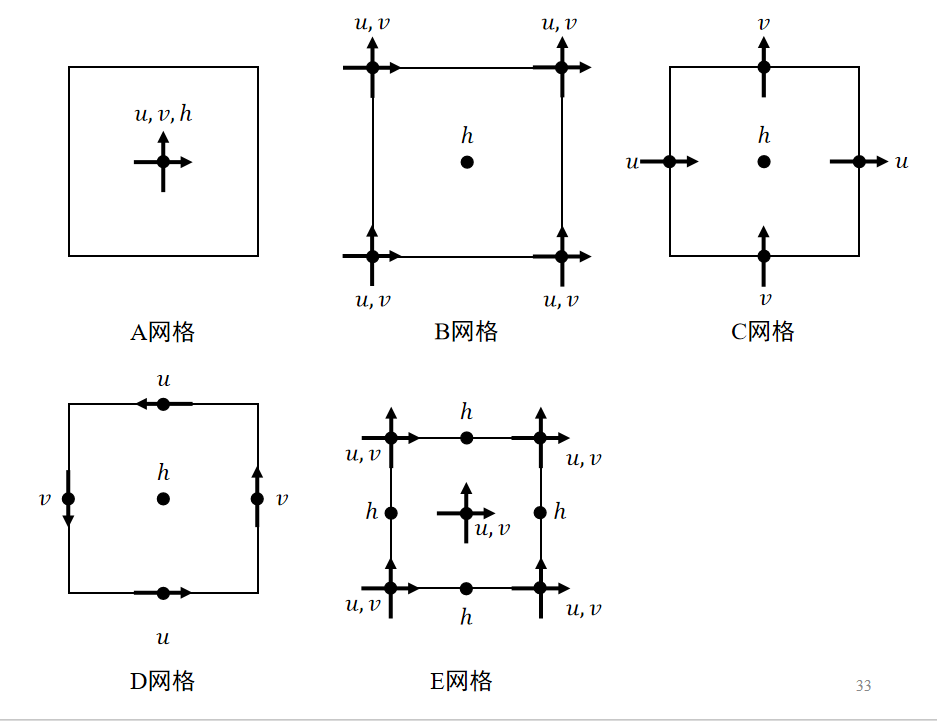
\includegraphics[width=\linewidth]{Fig3_3.png}
\end{center}

\subsubsection{ABCDE网格}

1. A网格存在气压模态,风场无法感受到气压梯度力,导致棋盘状扰动持久存在

2. B网格也存在类似A网格的气压模态

3. C网格在Rossby形变半径被网格很好解析时对惯性重力波描述最好

B网格在海洋模式应用广泛

C网格在大气应用广泛

C网格优点:

能够在网格距可以很好解析Rossby形变半径时较好刻画地转运动

消除虚假的气压和速度模态

C网格缺点:

科氏力计算需要平均风速,科氏力局地做功

\begin{center}
        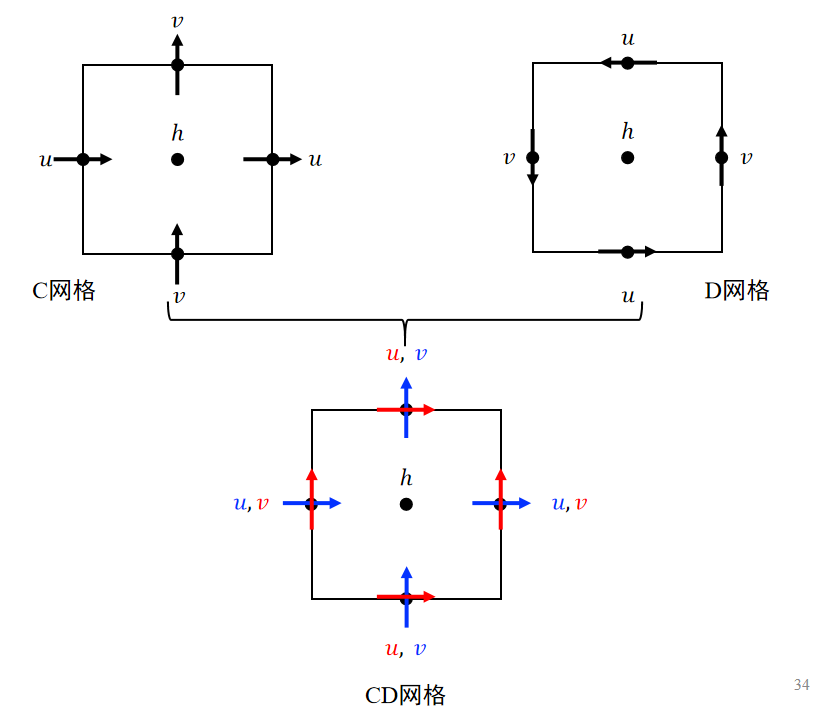
\includegraphics[width=\linewidth]{Fig3_4.png}
\end{center}

\subsection{平流方案}
平流方程是双曲型发展方程:

通量形式:
$$\frac{\partial \rho}{\partial t} + \nabla\cdot(\vec{u}\rho)=0$$

平流形式:
$$\frac{\partial q}{\partial t} +\vec{u} \cdot\nabla q=0$$

波动传播速度(即传播矩阵的特征值)是实数且有限,在平流方程中的传播速度即是流速。波动沿特征线传播$x=x_0+vt$

\subsubsection{频散项和耗散项}
耗散项具有偶数阶空间导数:
$$\frac{\partial f}{\partial t} = (-1)^{n+1}\alpha\frac{\partial^{2n} f}{\partial x^{2n}}$$

$\alpha>0$指数衰减,k越大,衰减越快;n越大,尺度选择性越高

频散项具有奇数阶空间导数
$$\frac{\partial f}{\partial t} = (-1)^{n+1}\alpha\frac{\partial^{2n} f}{\partial x^{2n}}$$

频散和耗散的推导:

1. 根据差分格式写出余项

2. 基于原平流方程得到时间导数和空间导数的关系,从而计算出最低阶的余项。

\subsubsection{时间前差空间中央差(FTCS)}
方程为反耗散,包含一个负粘性项,因此是绝对计算不稳定。
$$\frac{\rho^{n+1}_{i}-\rho^{n}_{i}}{\Delta t} + u \frac{\rho^{n}_{i+1} - \rho^{n}_{i-1}}{2 \Delta x} = 0$$

\subsubsection{二阶Lax-Wendroff格式(LW)}
该格式在时间前差-空间中央差格式的基础上,增加了一个正粘性项,以抵消前者中的负粘性项。从而变成频散方程。波数越大,传播越慢。
$$\frac{\rho^{n+1}_{i}-\rho^{n}_{i}}{\Delta t} + u \frac{\rho^{n}_{i+1} - \rho^{n}_{i-1}}{2 \Delta x} - \frac{u^2 \Delta t}{2} \frac{\rho ^n_{i+1}-2\rho^n_i+\rho^n_{i-1}}{\Delta x^2}= 0$$

\subsubsection{Crank-Nicolson方案(CN)}
该格式在时间前差-空间中央差的基础上,加入n+1时刻的空间差分,使得该格式为隐式;该格式同Lax-Wendroff格式一样也含有频散项。
$$\frac{\rho^{n+1}_{i}-\rho^{n}_{i}}{\Delta t} + \frac{u}{2}\left( \frac{\rho^{n+1}_{i+1} - \rho^{n+1}_{i-1}}{2 \Delta x}+\frac{\rho^{n}_{i+1} - \rho^{n}_{i-1}}{2 \Delta x}\right)= 0$$

\subsubsection{蛙跳格式}
该方案在时间前差-空间中央差格式的基础上,将时间前差变为中央差,因此需要三个时间层:
$$\frac{\rho^{n+1}_i-\rho^{n-1}_i}{2\Delta t} + u\frac{\rho^{n}_{i+1}-\rho^{n}_{i-1}}{2\Delta x}=0$$

蛙跳格式的余项:
$$\frac{\partial \rho }{\partial t} + u\frac{\partial \rho }{\partial x} = 
-\frac{u\Delta x^2}{6}\frac{\partial^3 \rho}{\partial x^3}$$

该方案同Lax-Wendroff方案一样不含有二阶扩散项,但却含有一个不与$\alpha$有关(与时间分辨率无关)的三阶频散项,因此会出现计算波,并且奇偶步会出现分离。

\subsubsection{一阶迎风格式}
修正方程包含一个正粘性项,因此是条件稳定。
$$\frac{\rho^{n+1}_{i}-\rho^{n}_{i}}{\Delta t} + \frac{u - |u|}{2} \frac{\rho^{n}_{i+1} - \rho^{n}_{i}}{\Delta x} + \frac{u + |u|}{2} \frac{\rho^{n}_{i} - \rho^{n}_{i-1}}{\Delta x}= 0$$


\subsubsection{Beam-Warming格式(BW)}
在一阶迎风格式的基础上采用二次多项式插值,也称二阶迎风格式。不同于一阶迎风格式,虽然也采用迎风方式计算通量,但是该格式含有频散项。波数越小,传播越慢
\begin{align}
    \frac{\rho^{n+1}_{i}-\rho^{n}_{i}}{\Delta t} &+ \frac{1}{2}\frac{u - |u|}{\Delta x} \left(-\frac{1}{2} (1 + \alpha) \rho^{n}_{i+2} + (2 + \alpha) \rho^{n}_{i+1} - \frac{1}{2} (3 + \alpha) \rho^{n}_{i} \right) \\
    &- \frac{1}{2} \frac{u + |u|}{2 \Delta x} \left(\frac{1}{2} (1-\alpha) \rho^{n}_{i-2} - (2-\alpha) \rho^{n}_{i-1} + \frac{1}{2} (3-\alpha) \rho^{n}_{i} \right)= 0
\end{align}

其中$\alpha = \frac{u\Delta t}{\Delta x}$


\subsubsection{精度壁垒(Godunov's theroem)}
Godunov(1959)证明没有比一阶更高的线性格式能够一直保证解的单调性(也称精度壁垒)。实用差分格式往往是非线性的(含有非线性滤波器)。

即:不能通过简单地提高近似阶数来降低频散误差,需要使用限制器等算法实现单调或正定。

有限差分方案主要是极力降低频散误差,保证解的正定性(单调性),同时又比迎风方案引入的扩散误差小
实用的欧拉或半拉格朗日方案一般为非线性


\subsubsection{通量订正方法FCT}
通量订正方法(Flux-Corrected Transport):主要思想是寻找单调性可能被打破的区域,然后采用某种方式避免虚假频散波动的发生。

通量订正方法的两种设计思路:

设计一种非线性的通量订正器(也称滤波器或限制器)

结合低阶格式和高阶格式的优点(也称混合方案)

\subsubsection{两步保形方案(TSPAS)}
两部保形方案(Transport Shape-Preserving Advection Scheme)

结合一阶迎风格式和二阶Lax-Wendroff格式。通过检测平流保形规则,设定修正速度,实现两种方案的切换。在平滑区域采用Lax-Wendroff格式,在不连续区域采用迎风格式,保证解的正定性。

1. 根据Lax-Wendroff格式计算一个临时量

2. 检查平流保形规则(Transport Shape-Preserving Advection Rule)

3. 根据临时量和所给的范围构造修正速度,用新的修正速度平流出最终结果。

\subsubsection{MPDATA方案}
与FCT类方案不同,对计算值进行迭代更正。基础格式是一阶迎风格式,每次迭代计算一个“反扩散速度”

\subsubsection{WENO方案}
对不同的计算模板做加权平均。

\subsubsection{有限体积方案}
一维双曲型波动方程(守恒律方程)可以写成微分形式和积分形式:

微分形式:
$$\frac{\partial q}{\partial t} +\frac{\partial f(q)}{\partial x}=0$$

积分形式:
$$\frac{1}{\Delta x}\int^{x_2}_{x_1}q(x,t_2)dx=\frac{1}{\Delta x}\int^{x_2}_{x_1}q(x,t_1)dt-\frac{1}{\Delta x}(\int^{t_2}_{t_1}q(x_2,t)dt-\int^{t_2}_{t_1}q(x_1,t)dt)$$

前者要求解光滑连续(强解),后者放宽了对解的限制(弱解)

前者求解的是点值,后者求解的是体元积分平均值

通过求解黎曼问题得到数值通量,并通过多种手段保证格式的精度和结果的无振荡

有限体积分方法的优点:

1. 一阶守恒量(总质量)自动守恒(有限差分也可以)

2. 从积分形式的出发方程上来说可以处理不连续性(计算流体中的激波)

3. 提高精度从提高重构函数的阶数出发即可,有多种通量限制器来避免高阶重构函数导致的频散误差

4. 便于应用于多边形网格(三角形、六边形)

有限差分与有限体积的异同:

1. 有限体积方案最终的计算形式与有限差分方案类似,甚至等价

2. 设计思路不同

3. 有限差分方案从Taylor展开出发,设计具有不同精度的差分格式

4. 有限体积方案从重构网格内分布出发,通过提高分布的近似度提高精度

5. 两种方案混合,既考虑重构,又考虑展开插值边界值


\subsubsection{黎曼问题}
\subsubsection{TVD格式和单调格式}
\subsubsection{FFSL方案}
\subsubsection{高阶迎风通量}
\subsubsection{WENO有限体积版本}
\subsubsection{Semi-Lagrange方案}
Semi-Lagrange方案主要解决欧拉方案存在的严格时间步长的限制。

时间步长的选取应该主要受制于精度,而非稳定性。Semi-Lagrange方案时间步长可以大一个量级。同时绕过了Lagrange方案需要解决的流体大形变问题

追踪点的Semi-Lagrange方案:

追踪面积的Semi-Lagrange方案:(CSLAM方案)

\subsubsection{Lagrange方案}
半拉格朗日方案解决了欧拉方案存在的严格时间步长限制,并且追踪面积的半拉格朗日方案解决了质量守恒问题,但是数值扩散误差却仍然很大。

同Semi-Lagrange方案类似,但是始终追踪微团,而不是每步重置到网格单元

最大优点:极大减少欧拉和半拉格朗日方案中存在的扩散误差

连续示踪物被离散为有限个数的微团,不受固定网格限制,完全二维或三维,同时时间步长限制小。全拉格朗日方案不受网格限制,追踪示踪物微团,因此能够极大降低由于网格分辨率不足导致的扩散误差

混淆误差:流场的巨大形变性使得难以描述微团的形状,极大影响数值计算精度。离散微团所代表的空间范围没有模拟好,产生混淆误差。

\section{垂直坐标}
高度z坐标:

优点:

简单直观

坐标面不随时间变化

缺点:

与地形相交,产生小网格

等高面与等压面或等位势密度面不重合,容易产生虚假的数值混合

一般会结合阶梯地形或地形追随坐标改造

\subsection{物理量坐标}
均与地形相交,形成复杂的下边界,较难用于模式计算
\subsubsection{气压p坐标}
使用气压p作为垂直坐标(Surcliffe,1947)。以静力平衡为前提条件:$\partial p/\partial z=−\rho g$

气压p坐标的优点:
\begin{itemize}
    \item 方程形式简单,水平气压梯度力(PGF)不显含密度,地转风计算简单
    \item 连续方程简化
    \item 便于与传统天气分析结合做预报:天气图正是在等压面上绘制的
\end{itemize}

气压p坐标的缺点:(下边界条件复杂)
\begin{itemize}
    \item 地面不是一个坐标面
    \item 垂直层随时间变化:p(x,y,z,t)
\end{itemize}

\subsubsection{静力气压pi坐标}
为了便于静力模式与非静力模式对比,使用静力气压$\pi$作为垂直坐标(Laprise,1992),也称质量坐标:
$$\pi(x,y,z,t)=\pi_T+\int^{z_T}_{z}{\rho(x,y,z^{\prime},t)g} dz^{\prime}$$

用于大气模式WRF

\subsubsection{位温theta坐标}
用位温作为垂直坐标(Charney and Phillips,1953):
$$\theta=T(\frac{p_0}{p})^{\frac{R}{c_p}}$$

适用于锋面和急流区域

用于行星大气模式EPIC

优点:
\begin{itemize}
    \item 能增加锋面和对流层顶的垂直分辨率
    \item 对于绝热运动,气流沿着等位温面运动,减少“垂直速度”的计算误差和“垂直平流”的计算开销
    \item 垂直速度完全由非绝热加热产生
    \item 能保持位涡守恒
\end{itemize}

缺点:
\begin{itemize}
    \item 坐标面与地面相交
    \item 随高度的增加,不是单调变化,特别是在边界层
    \item 在绝热层,垂直分辨率较低
\end{itemize}

\subsubsection{位势密度rho坐标}
为了克服高度坐标跨坐标面运动产生的虚假数值混合,用(位)密度作为垂直坐标。用于海洋模式MICOM(Miami Isopycnic Coordinate Ocean Model)和NLOM(Navy Layered Ocean Model),这类模式也成layer model。


优点:
\begin{itemize}
    \item 易于描述层结海洋,控制跨等密度面混合
    \item 在密度变化大区域分辨率高
\end{itemize}

缺点:
\begin{itemize}
    \item 在中性层结区域分辨率低
    \item 对平流方案正定性要求高(不能出现负质量)
\end{itemize}

\subsection{地形追随坐标系}
通过变换将地面变成一个坐标面(模式面),为模式提供简单的下边界条件。
\subsubsection{基于气压p的地形追随坐标}
Phillips于1957年最早提出基于气压p的地形追随坐标($\sigma$坐标)
$$\sigma = \frac{p-p_t}{p_s-p_t}$$

其中$p_t$为模式顶的气压top,$p_s$为地面气压surface。

\subsubsection{基于高度的地形追随坐标}
Gal-Chen和Somerville于1975年提出基于高度的$\sigma$坐标
$$Z(x,y,z) = H\frac{z-h}{H-h}$$

H是模式层顶的高度,h是地形高度。量纲仍为高度。

Blumberg和Mellor(1980,1987)在海洋模式中使用了基于高度的$\sigma$坐标
$$\sigma = \frac{z-\eta}{H+\eta}$$

H是海底地形的深度,$\eta$是海表抬升高度,量纲为1。

坐标面坡度的空间变化:地形坡度越大,坡度越大;地形高度越大,坡度越大;坐标高度越高,坡度越小。

\subsubsection{两大计算误差}
\begin{center}
        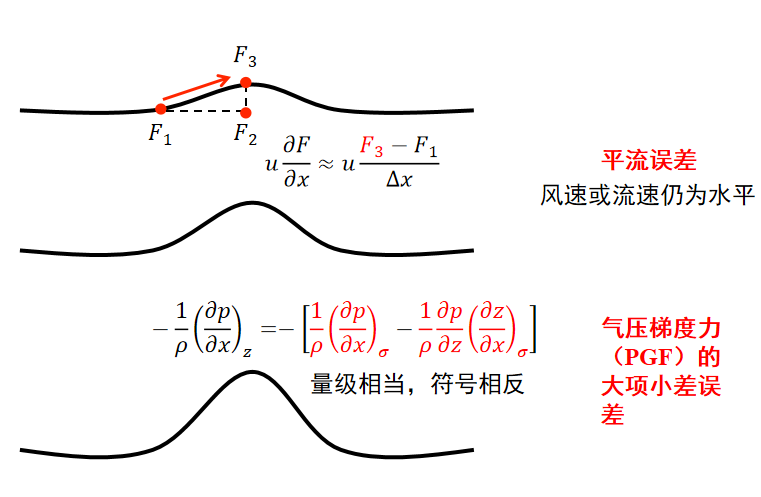
\includegraphics[width=0.8\linewidth]{Fig4_1.png}
\end{center}

1. 平流误差

由于坐标系非正交,导致存在平流误差。在陡峭地形附近,由于存在气压梯度和平流误差,导致风场误差。平滑地形,导致温度和湿度误差,也不利于同化近地面观测

2. PGF(Pressure Gradient Force)误差

\subsubsection{气压梯度力误差的解决方法}
1. 设计PGF计算方案,提高计算精度

减少大项小差:特殊差分格式,扣除法

避免大项小差:坐标变换法,有限体积法,谱近似方法

2. 修正PGF计算结果,减少计算误差

误差扣除法,误差增量表达式控制法,粘性系数订正法,网格调整法


\section{分裂算法}

\section{资料同化方法}
分析资料是日常数值天气预报业务中采用当前的同化系统和预报模式实时同化当前所能获取的多源观测资料而产生的大气或海洋当前状况的最优估计,用作模式初值;

在较长时期,同化系统和预报模式可能会更新或升级,不是固定不变的,同化的观测资料由于预报时效的限制也不是最全的。

再分析资料则是采用同一个的比较成熟的同化系统和预报模式在较长历史时期内同化所有能获取的多源观测资料而产生的大气或海洋状况最优估计的历史时间序列;

针对较长历史时期,同化系统和预报模式是固定不变的,同化的观测资料由于没有预报时效的限制是最完整的。

数据同化:

是在现有观测技术水平下,有效利用所能获取的各种观测数据和预报背景场,产生规则网格上的最优(再)分析数据,其误差理论上既小于观测误差也小于背景误差,是整体提高数值预报/预测技巧的关键技术之一;

影响同化性能的因素主要包括:

同化方法

初猜场的质量(预报误差)

观测资料的质量控制与误差的估计

观测策略


\subsection{资料同化的三大理论基础}
最小方差最小化观测的权重,而最大似然估计和贝叶斯理论则最小化观测本身;

分析误差方程的最小化、似然估计的最大化与代价函数的最小化等价;

三个理论都假定观测资料和先验估计的误差是无偏的,服从高斯分布。

最小方差估计:最优插值和卡曼滤波

最大似然估计和贝叶斯理论:三维和四维变分

\subsubsection{最小方差估计}
用多个观测值的方差估计真值,方差代表观测值到真值的距离。

假设对于多个独立的观测:
$$T_n = T_t + \varepsilon_n, \varepsilon_n\sim F_n(0, \sigma^2_n)$$

假定仪器的测量值是无偏的,知道观测误差方差,假定观测误差不相关,则用多个观测值的线性组合:
$$T_a = \Sigma a_n T_n$$

可得:
$$\Sigma a_n = 1$$
$$\Sigma a_n^2 \sigma_n^2 = \sigma_a^2$$

求方差极小得到:
$$a_n = \frac{1}{\sigma_n^2}\Sigma_{i\ne n} a_i\sigma_i^2$$

求解这个矩阵可以得到最小方差估计的权重。

\subsubsection{最大似然估计}
构造代价函数,代价函数极小为最优估计。

假设对于多个独立的观测:
$$T_n = T_t + \varepsilon_n, \varepsilon_n\sim F_n(0, \sigma^2_n)$$

似然函数就是观测为真值的概率的联合概率密度函数:
$$L = \Pi P_n(T_t, T_n, \sigma_n)$$

我们假设观测服从高斯分布,可以得到似然函数极大,就是解最逼近真值的结果:
$$J(T) = min[\Sigma \frac{T-T_n}{2\sigma_n^2}]$$

对应数据同化里的代价函数:
$$J(x) = \frac{1}{2}(x-x_b)^{T}B^{-1}(x-x_b) + \frac{1}{2}(H(x)-y_{obs})^{T}R^{-1}(H(x)-y_{obs})$$

从而得到变分同化方法。

\subsubsection{贝叶斯理论}
构造后验概率,后验概率极大为最优估计。

假设对于多个独立的观测:
$$T_n = T_t + \varepsilon_n, \varepsilon_n\sim F_n(0, \sigma^2_n)$$

我们假设观测服从高斯分布,可以得到后验概率极大,就是解最逼近真值的结果:
$$J(T) = min[\Sigma \frac{T-T_n}{2\sigma_n^2}]$$

\subsection{最优差值OI}
最优插值是利用最小方差估计把带有误差的观测资料有机地融合到模式预报所得到的背景场中,从而得到对模式初值的最优估计。

我们考虑分析场:
$$x_a = x_b + W[y_{obs} - H(x_b)]$$

假定观测算子是线性的:
$$x_a = x_b + W[y_{obs} - H(x_b)] =  x_b + W[y_{obs}-H(x_t)+H(x_t)-H(x_b)]=x_b + W[\varepsilon_o-H\varepsilon_b]$$

根据$\nabla_W \sigma_a = 0$,解得
$$W = BH^T(R + HBH^T)^{-1}$$

这里的B即背景误差协方差矩阵:
$$B=\overline{\varepsilon_b\varepsilon_b^T}$$

R为观测误差协方差矩阵:
$$R=\overline{\varepsilon_o\varepsilon_o^T}$$

在实际计算中,背景场和观测场往往不是无偏的,因此,B和R要做无偏处理:
$$B=\overline{(\varepsilon_b-\overline{\varepsilon_b})(\varepsilon_b-\overline{\varepsilon_b})^T}$$
$$R=\overline{(\varepsilon_o-\overline{\varepsilon_o})(\varepsilon_o-\overline{\varepsilon_o})^T}$$

在OI中假定,背景误差和观测值误差不相关。在实际分析中,这种假设是完全合理的,因为背景误差的成因和观测值误差的成因是完全独立的。

但实际分析中,观测预处理过程(如卫星资料的反演)会用到背景场信息,使得观测误差的估计包含背景误差信息,导致OI的近亲繁殖问题(incest problem),这样难以得到最优分析。

最优差值的特点:

1、权重矩阵W主要不依赖于分析格点的位置;

2、观测误差方差较大的观测资料将获得较小的权重;

3、对背景误差协方差更大的分析格点,观测资料将获得更大的权重,对分析产生更大的影响。  

4、OI比逐步订正法更合理,但代价是要求解一个PxP阶的逆矩阵或P阶线性方程组(P为观测个数)

5、进行大尺度流场分析时,若在背景误差协方差引入地转关系,可避免独立估计风场的误差相关,强制保持风场和位势场分析增量的近似地转,改进其平衡关系。


\subsection{背景误差协方差}
由于真值$x_t$并不知道,也就不知背景误差和观测误差,因此只能用它们统计特征。如果背景和观测值有偏,原则上使用资料前要进行校正。

如果偏差保留在同化过程中,那么分析肯定不是最优的,所以监控偏差非常重要,主要通过分析背景场误差(background departure )的平均,但是很难判断这种偏差是模式偏差还是观测偏差,这也是资料同化的热点研究问题。

背景误差(协)方差统计不对,会导致分析增量过大或过小,不但背景误差和观测误差方差比值重要,背景误差的绝对数值也很重要,背景误差大,同化系统更容易吸收观测。

\subsubsection{背景误差协方差的作用}
背景误差协方差矩阵(B)是否随着天气形势而演变,即流依赖(flow-dependent)特征,是衡量同化方法好坏的重要指标之一。

1、信息传递(information spreading):资料稀缺区域,分析增量的形状完全由协方差结构决定的,由B的相关性决定了从观测点到它周围的区域的信息空间传播

2、信息平滑(information smoothing):资料稠密区域,B的相关性决定观测信息的平滑程度,分析增量平滑使得其与物理场平滑是相匹配的。

3、平衡特征(balance properties):实际大气存在某种平衡,背景误差协方差应该体现这种平衡,例如大尺度运动通常是地转平衡的,观测到一种模式变量位势高度,可以根据扰动量的地转平衡关系分析风场增量信息。

\subsubsection{背景误差协方差的估计}
1. HL(Holligsworth-Lonnberg)方法

利用短期预报与观测(如无线电测风)的差值来估计,该方法要求观测足够密,足够多,尽可能是独立的观测。

2. NMC(National Meteorological Center)方法

利用滞后的历史预报样本来估计背景误差,假设模式对初值的敏感性和背景误差成正比。
$$x_1^k(t) = M_{24}x_a^{k}(t-24)$$
$$x_2^k(t) = M_{48}x_a^{k}(t-48)$$
$$\varepsilon_b^{k} = x_1^k - x_2^k$$

其中k为第k个采样,每个采样前进一段时间步长,用模式对不同初始场在相同位置的预报差作为背景误差。得到:
$$b = \frac{1}{\sqrt{n_s - 1}}(\varepsilon^k_b - \overline{\varepsilon_b})$$


3. 集合预报方法(Ensemble Forecast)

利用预报模式基于多初值对同一时刻的预报样本,来统计B矩阵,其中这些预报样本的集合平均作为真值的期望。

用NMC方法一般基于历史预报样本,因此统计出来的B矩阵往往是静态的,不随天气演变而改变,即不具有流依赖特征,不利于同化能力的充分发挥;

集合预报方法则是用最近的预报样本,甚至即时生成预报样本,这些样本是随天气演变而改变的,具有流依赖特征,利于提高同化的能力。

\subsubsection{局地化和平衡性}
无论是用NMC方法还是集合预报方法,统计出来的B矩阵是一个奇异矩阵,这样B的逆矩阵不存在,会使得OI的权重系数无法计算,同样也会影响到后面要讲到的变分同化的实施。主要原因是误差样本或预报样本的维数很高,如前面所说,可达到$10^7~10^8$量级,而取样个数是无论如何也达不到这么大的数量。NMC方法一般才$10^3$量级的样本数,而集合预报方法的样本数更少($10^1~10^2$量级)。

局地化是缓解B矩阵不满秩问题的有效方法;

用NMC方法统计的B矩阵,一般采用递归滤波法对水平方向进行局地化,用EOF分解对垂直方向进行局地化;用集合预报方法统计的B矩阵,一般用一个在滤波半径内随指数衰减,之外为0的相关矩阵与B矩阵进schür乘积。

局地化往往会破坏B矩阵的平衡约束,为了解决这个问题,局地化应该只针对非平衡部分进行;

把控制变量分解成平衡部分和非平衡部分,并利用非平衡部分组成新控制变量,并通过对它们做物理变换变回原来的控制变量;

针对新的控制变量建立新的B矩阵,对新的B矩阵做局地化,这样同化后得到新控制变量的分析场,然后通过物理变换得到原来控制变量的分析场。

\subsection{变分同化}
\subsubsection{共轭梯度法}
\subsubsection{3Dvar同化}

在同化问题中有三个关键的误差(背景误差、观测误差和模式误差),而这些误差不能准确的估计,导致同化问题的解是统计意义上的。

通过给出极大似然函数,得到分析场是真值的极大似然解。从而资料同化变为一个目标函数的极小化问题:
$$J(x) = \frac{1}{2}(x-x_b)^{T}B^{-1}(x-x_b) + \frac{1}{2}(H(x)-y_{obs})^{T}R^{-1}(H(x)-y_{obs})$$

解得:
$$x_a = x_b + (B^{-1} + H^TR^{-1}H)^{-1}H^TR^{-1}(y_{obs} - Hx_b)$$

类似OI最优插值,有:
$$W_{3Dvar} = (B^{-1} + H^TR^{-1}H)^{-1}H^TR^{-1}$$

对比OI有:
$$W_{OI} = BH^T(R + HBH^T)^{-1}$$

不难得到,两者本质上等价,但由于解法不一样,结果并不相同。

观测资料个数远远小于模式的维数,将3DVar的极小化变换到观测值(物理)空间(Da Silva等1995),叫物理空间分析方案,也叫3DVar的双公式方案。

模式空间:
$$\delta x_a=(B^{-1} + H^TR^{-1}H)^{-1}H^TR^{-1}\delta y_a$$

物理空间:
$$\delta x_a = BH^T(R + HBH^T)^{-1}y_a$$

由于观测空间的维度较小,物理空间上的方程计算量要更小,而且不需要多次求解逆矩阵。从而在物理空间上最小化问题。

第一步,求解线性方程组:
$$(R + HBH^T)w = y_a$$

对于Ax=b,当A为正定矩阵时,方程的解是函数$\phi(x) = \frac{1}{2}x^TAx - b^Tx$的极小值点。

第二步:
$$\delta x_a = BH^T w$$

3DVar用全局最优化算法,不需要挑选观测资料,所有观测同时被使用,避免了不同资料选择区边界上的不连续。

增量法:
$$J(x) = \frac{1}{2}(x-x_b)^{T}B^{-1}(x-x_b) + \frac{1}{2}(H(x)-y_{obs})^{T}R^{-1}(H(x)-y_{obs})$$
$$J(\delta x) = \frac{1}{2}(\delta x)^{T}B^{-1}(\delta x) + \frac{1}{2}(H(\delta x)-d)^{T}R^{-1}(H(\delta x)-d)$$

从而:
$$x_n = x_{n-1} + S^{-1}\delta x_n$$

S:高分辨率模式空间到低分辨率模式空间的变换算子(插值或截谱)。外循环迭代分析场,内循环根据代价函数更新分析增量。

这种方法不但降低计算代价,而且通过保持线性化的观测算子H,在“内”迭代为常数,而在“外”迭代中更新的办法,把目标函数求极小时观测算子中观测与模式变量间的重要的非线性关系结合起来了。

\subsubsection{4Dvar同化}
四维变分的代价函数形式:
$$J(x) = \frac{1}{2}(x-x_b)^{T}B^{-1}(x-x_b) + \frac{1}{2}\Sigma_i(HM_{t_0\longrightarrow t_i}x-y^i_{obs})^{T}R_i^{-1}(HM_{t_0\longrightarrow t_i}x-y^i_{obs})$$

增量形式:
$$J(\delta x) = \frac{1}{2}(\delta x)^{T}B^{-1}(\delta x) + \frac{1}{2}\Sigma_i(HM_{t_0\longrightarrow t_i}\delta x-d^i)^{T}R_i^{-1}(HM_{t_0\longrightarrow t_i}\delta x-d^i)$$

\subsection{Kalman滤波}
\subsubsection{Kalman滤波}
\subsubsection{集合Kalman滤波}
\begin{table}[h!]
  \begin{center}
    \caption{三种同化方式的比较}
    \begin{tabular}{c|c|c|c} 
      \textbf{指标} & \textbf{3DVar/OI} & \textbf{4DVar} & \textbf{EnKF}\\
      \hline
      B矩阵 & 模型化,不随流发展 & 模型化,窗口内隐式流依赖 & 非模型化,全局显式流依赖 \\
      关键技术 & 伴随 & 伴随 & 集合\\
      同化方式 & 顺序、非全局最优 & 非顺序、全局最优 & 顺序,非全局最优\\
      与模式协调性 & 较好 & 好 &  较好\\
      开发难度&中&大&小\\
      计算量&小&很大&大\\
      并行效率&一般&低&高\\
      滤波发散&无&无&有
    \end{tabular}
  \end{center}
  \end{table}

\subsection{切线性模式和伴随模式}
必要性与困难
\begin{itemize}
    \item 目标函数的极小化无论采用线性共轭梯度法还是非线性共轭梯度法(如L-BFGS方法)均需要伴随观测算子,4DVar还需要伴随模式;
    \item 大气、海洋模式非常复杂,是非线性的和高维的,无法显式表示,更无法用矩阵变换的方式把模式表示出来;
    \item 切线性模式也只能以矩阵与向量相的方式存在,无法将G显式表示。
\end{itemize}

三种不同生成切线性和伴随程序的方法
\begin{itemize}
    \item 从原微分方程出发,写出切线性方程和伴随方程,然后对它们离散,再编写程序;
    \item 从计算格式出发,写出其对应的切线性格式和伴随格式,然后再编程;
    \item 从计算格式的程序代码出发,直接编写切线性程序和伴随程序的代码。
\end{itemize}

\subsubsection{切线性模式的编写}

直接基于原子程序进行编写,其规则如下:

1. 搞清楚原子程序的输入、输出变量,并开辟对应的扰动数组;

2. 原子程序的代码全部保留,并在每条与输入输出有关赋值语句的上方编写切线性代码,采用对赋值语句进行微分的法则来编写;

3. 循环语句和条件语句本身保持不变

\subsubsection{伴随模式的编写}
参考切线性程序进行编写,其规则如下:

1. 伴随子程序应与切线性子程序有相同的亚元变量表,
但输入输出变量正好与切线性代码相反;

2. 循环语句一般相对于相应的切线性代码是反序的;

3. 伴随子程序的所有输出变量和中间工作变量在开始
时全部清零;

4. 赋值语句采用叠加形式,如“x=x+a”;

5. 在伴随代码前面,复制完整或主要的原子程序代码,以保留伴随代码所需要的基态变量的值,保留的方式可以开数组变量保留,也可以用硬盘存贮;

6. 伴随代码的编写应参照切线性代码从其尾部往前写,顺序完全与切线性代码相反。

\subsection{混合同化方法}
混合资料同化能够在集合和变分两种同化方法之间取长补短,发挥出更大的优势,因而成为资料同化领域的国际前沿。

\subsubsection{En3DVar}
\subsubsection{En4DVar}
\subsubsection{4DEnVar}
利用集合样本的统计关系替代了切线性模式和伴随模式,从而大大减轻了开发难度、降低了计算量,这是实现4DVar一种非常高效的方式;

\subsection{耦合资料同化}
非耦合资料同化:我们前面介绍的最优插值、变分同化、集合同化和混合同化等方法,均是采用非耦合模式(如单独大气模式或单独海洋模式)的预报作为背景场(先验估计),这样的同化方法均属于非耦合资料同化;

耦合资料同化:无论哪种资料同化方法,若其背景场是采用多圈层耦合模式的预报,则称之为耦合资料同化。

根据世界天气研究计划的定义,耦合资料同化指的是在多圈层耦合的地球系统模式(简称“耦合模式”)框架下进行的资料同化,能应用于耦合模式中每个单独分量模式(称为弱耦合资料同化),或把耦合模式作为一个整体进行同化(称为强耦合资料同化)(Penny et al, 2017);

与耦合同化相对应,非耦合资料同化是指针对某个单独分量模式的单圈层同化,如当前用于数值天气预报系统的针对单独大气模式的资料同化。



\end{document}
